\documentclass[12pt, a4paper]{article}
\usepackage{../../../myconfig_line} % Gọi file cấu hình từ ngoài gốc vào
% ==========================================
% BẮT ĐẦU NỘI DUNG TÀI LIỆU
% ==========================================
\begin{document}

% Truyền 3 tham số: {Nhãn cam} {Chữ to chính giữa} {Chữ ở góc phải Header}
\titlebox{Chủ đề: Tích phân}{Ứng dụng tích phân trong bài toán chuyển động}{Bài toán chuyển động}

% --- CÂU 1 ---
\questionTrueFalse{20}{1}{Một chất điểm bắt đầu chuyển động thẳng đều với vận tốc \(v_0\), sau 5 giây chuyển động thì gặp chướng ngại vật nên bắt đầu giảm tốc độ với vận tốc chuyển động \(v(t) = -3t + a\) (m/s), (\(t \geq 5\)) cho đến khi dừng hẳn. Quãng đường chất điểm đi được kể từ lúc chuyển động đến khi dừng hẳn là \(\dfrac{200}{3}\) m.}{
    \textbf{a)} & Quãng đường chất điểm đi chuyển được sau 5 giây bằng \(S(5) = 5v_0\) (m).
    & \textcolor{amberorange}{$\bigcirc$} & \textcolor{amberorange}{$\bigcirc$} \\ \hline
    
    \textbf{b)} & Quãng đường chất điểm đi chuyển được sau 7 giây bằng \(S(7) = \displaystyle\int_{0}^{7} v(t) dt\) (m).
    & \textcolor{amberorange}{$\bigcirc$} & \textcolor{amberorange}{$\bigcirc$} \\ \hline
    
    \textbf{c)} & \(v_0 < 8\) (m/s).
    & \textcolor{amberorange}{$\bigcirc$} & \textcolor{amberorange}{$\bigcirc$} \\ \hline
    
    \textbf{d)} & Vận tốc trung bình \(v_{tb}\) của chất điểm trong khoảng thời gian từ 2 giây đến 7 giây kể từ lúc bắt đầu thỏa mãn \(v_{tb} < 8\) (m/s).
    & \textcolor{amberorange}{$\bigcirc$} & \textcolor{amberorange}{$\bigcirc$} \\
}




% --- CÂU 2 ---
\questionTrueFalse{25}{2}{Một người điều khiển ô tô đang ở đường dẫn muốn nhập làn vào đường cao tốc. Khi ô tô cách điểm nhập làn 200 m, tốc độ của ô tô là 54 km/h. Hai giây sau đó, ô tô bắt đầu tăng tốc với tốc độ \(v(t) = at + b\) (\(a, b \in \mathbb{R}; a > 0\)), trong đó \(t\) là thời gian tính bằng giây kể từ khi bắt đầu tăng tốc. Biết rằng ô tô nhập làn cao tốc sau 10 giây tăng tốc và duy trì sự tăng tốc trong 20 giây kể từ khi bắt đầu tăng tốc, sau 20 giây đó ô tô duy trì tốc độ cao nhất trong 24 giây đầu trong thời gian còn lại trên cao tốc.}{
    \textbf{a)} & Quãng đường ô tô đi được từ khi bắt đầu tăng tốc đến khi nhập làn là 170 m.
    & \textcolor{amberorange}{$\bigcirc$} & \textcolor{amberorange}{$\bigcirc$} \\ \hline
    
    \textbf{b)} & Vận tốc của ô tô tại thời điểm nhập làn là 72 km/h.
    & \textcolor{amberorange}{$\bigcirc$} & \textcolor{amberorange}{$\bigcirc$} \\ \hline
    
    \textbf{c)} & Quãng đường mà ô tô đi được trong thời gian 30 giây kể từ khi ô tô cách điểm nhập làn 200 m là 594 m.
    & \textcolor{amberorange}{$\bigcirc$} & \textcolor{amberorange}{$\bigcirc$} \\ \hline
    
    \textbf{d)} & Sau 20 giây kể từ khi tăng tốc, ô tô duy trì tốc độ cao nhất trong vòng 6 giây thì phát hiện chướng ngại vật cách ô tô 200 m, người điều khiển lập tức đạp phanh và ô tô chuyển động chậm dần đều với \(a(t) = -3\) (m/s\(^2\)). Khi đó ô tô dừng lại cách chướng ngại vật 10 m.
    & \textcolor{amberorange}{$\bigcirc$} & \textcolor{amberorange}{$\bigcirc$} \\
}


% --- CÂU 3 ---
\questionShortAnswer{30}{3}{Một ô tô đang chạy với vận tốc 12 m/s thì người lái xe đạp phanh. Từ thời điểm đó, ô tô chuyển động chậm dần đều với vận tốc \(v(t) = -2t + 12\) (m/s), trong đó \(t\) là khoảng thời gian được tính bằng giây, kể từ lúc bắt đầu đạp phanh. Quãng đường ô tô di chuyển được trong 10 giây cuối cùng bằng bao nhiêu? (làm tròn kết quả đến hàng đơn vị).
}

% --- CÂU 4 ---
\questionShortAnswer{30}{4}{Một xe ô tô đang chạy với vận tốc 20 m/s thì xe bắt đầu giảm tốc độ để tránh va chạm với chướng ngại vật ở phía trước với vận tốc cho bởi công thức \(v(t) = at + b\) (\(a, b \in \mathbb{R}\)) trong đó \(t\) là thời gian tính bằng giây kể từ khi bắt đầu giảm tốc. Sau 5 giây thì xe dừng hẳn trước chướng ngại vật. Quãng đường từ khi bắt đầu giảm tốc độ đến khi xe dừng hẳn là bao nhiêu mét?
}

% --- CÂU 5 ---
\questionShortAnswer{25}{5}{Một xe ô tô sau khi chờ hết đèn đỏ, bắt đầu chuyển động trong 6 phút đầu với vận tốc được biểu thị bằng một phần đường cong parabol, sau đó ô tô chuyển động đều với vận tốc được biểu thị bởi một phần đường thẳng và được mô tả như hình vẽ. Biết rằng trong 6 phút đầu thì xe đạt đến vận tốc cao nhất là 1000 (mét/phút). Hỏi quãng đường xe đã đi được trong khoảng 10 phút đầu tiên là bao nhiêu mét?

\begin{center}
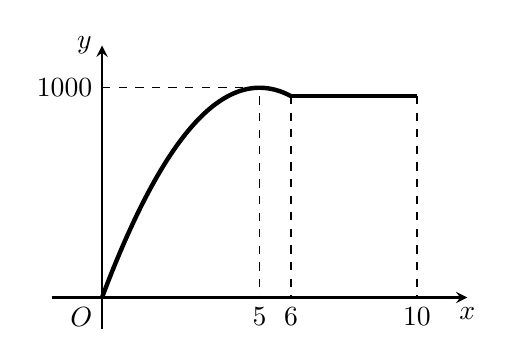
\begin{tikzpicture}[scale=0.8, >=stealth]
    % Tỉ lệ: x = x_thật / 2, y = y_thật / 300
    % x=0 (0,0)
    % x=5 (2.5, 3.33) [y=1000]
    % x=6 (3.0, 3.20) [y=960]
    % x=10 (5.0, 3.20) [y=960]

    % Trục tọa độ
    \draw[->, thick] (-0.8, 0) -- (5.8, 0) node[below] {$x$};
    \draw[->, thick] (0, -0.5) -- (0, 4.0) node[left] {$y$};

    % Gốc tọa độ O
    \node[below left] at (0,0) {$O$};

    % Đường đứt nét (Dashed lines)
    \draw[dashed] (0, 3.33) node[left] {$1000$} -- (2.5, 3.33) -- (2.5, 0) node[below] {$5$};
    \draw[dashed] (3.0, 3.20) -- (3.0, 0) node[below] {$6$};
    \draw[dashed] (5.0, 3.20) -- (5.0, 0) node[below] {$10$};

    % Đồ thị
    % Parabol: y = -40(x-5)^2 + 1000 trong đoạn [0, 6]
    \draw[ultra thick, domain=0:3.0, samples=100] 
        plot (\x, {(-\x*\x +5*\x)*333/625});

    % Đoạn thẳng nằm ngang từ x = 6 đến x = 10
    \draw[ultra thick] (3.0, 3.20) -- (5.0, 3.20);

\end{tikzpicture}
\end{center}
}

\end{document}